
% v2-acmsmall-sample.tex, dated March 6 2012
% This is a sample file for ACM small trim journals
%
% Compilation using 'acmsmall.cls' - version 1.3 (March 2012), Aptara Inc.
% (c) 2010 Association for Computing Machinery (ACM)
%
% Questions/Suggestions/Feedback should be addressed to => "acmtexsupport@aptaracorp.com".
% Users can also go through the FAQs available on the journal's submission webpage.
%
% Steps to compile: latex, bibtex, latex latex
%
% For tracking purposes => this is v1.3 - March 2012
\documentclass[prodmode,acmtecs]{acmsmall} % Aptara syntax
\usepackage[spanish,polish]{babel}
\usepackage[T1]{fontenc}
\usepackage{fancyvrb}
\usepackage{graphicx,hyperref}
\newcommand\cutout[1]{}


\usepackage[table]{xcolor}
\usepackage[utf8]{inputenc}
\usepackage[parfill]{parskip}
\usepackage{tabulary}
\PassOptionsToPackage{hyphens}{url}
\usepackage{hyperref}    
\usepackage[capitalize]{cleveref}


% Metadata Information
% !!! TODO: SET THESE VALUES !!!
\acmVolume{0}
\acmNumber{0}
\acmArticle{CFP}
\acmYear{0}
\acmMonth{0}

\newcounter{colstart}
\setcounter{page}{4}

\RecustomVerbatimCommand{\VerbatimInput}{VerbatimInput}%
{
%fontsize=\footnotesize,
fontfamily=\rmdefault
}


\newcommand{\UnderscoreCommands}{%\do\verbatiminput%
\do\citeNP \do\citeA \do\citeANP \do\citeN \do\shortcite%
\do\shortciteNP \do\shortciteA \do\shortciteANP \do\shortciteN%
\do\citeyear \do\citeyearNP%
}

\usepackage[strings]{underscore}



% Document starts
\begin{document}


\setcounter{colstart}{\thepage}

\acmArticle{CFP}
\title{\huge\sc SIGLOG Monthly 213}
\author{DAVID PURSER\affil{Max Planck Institute for Software Systems, Saarbr\"ucken}
\vspace*{-2.6cm}\begin{flushright}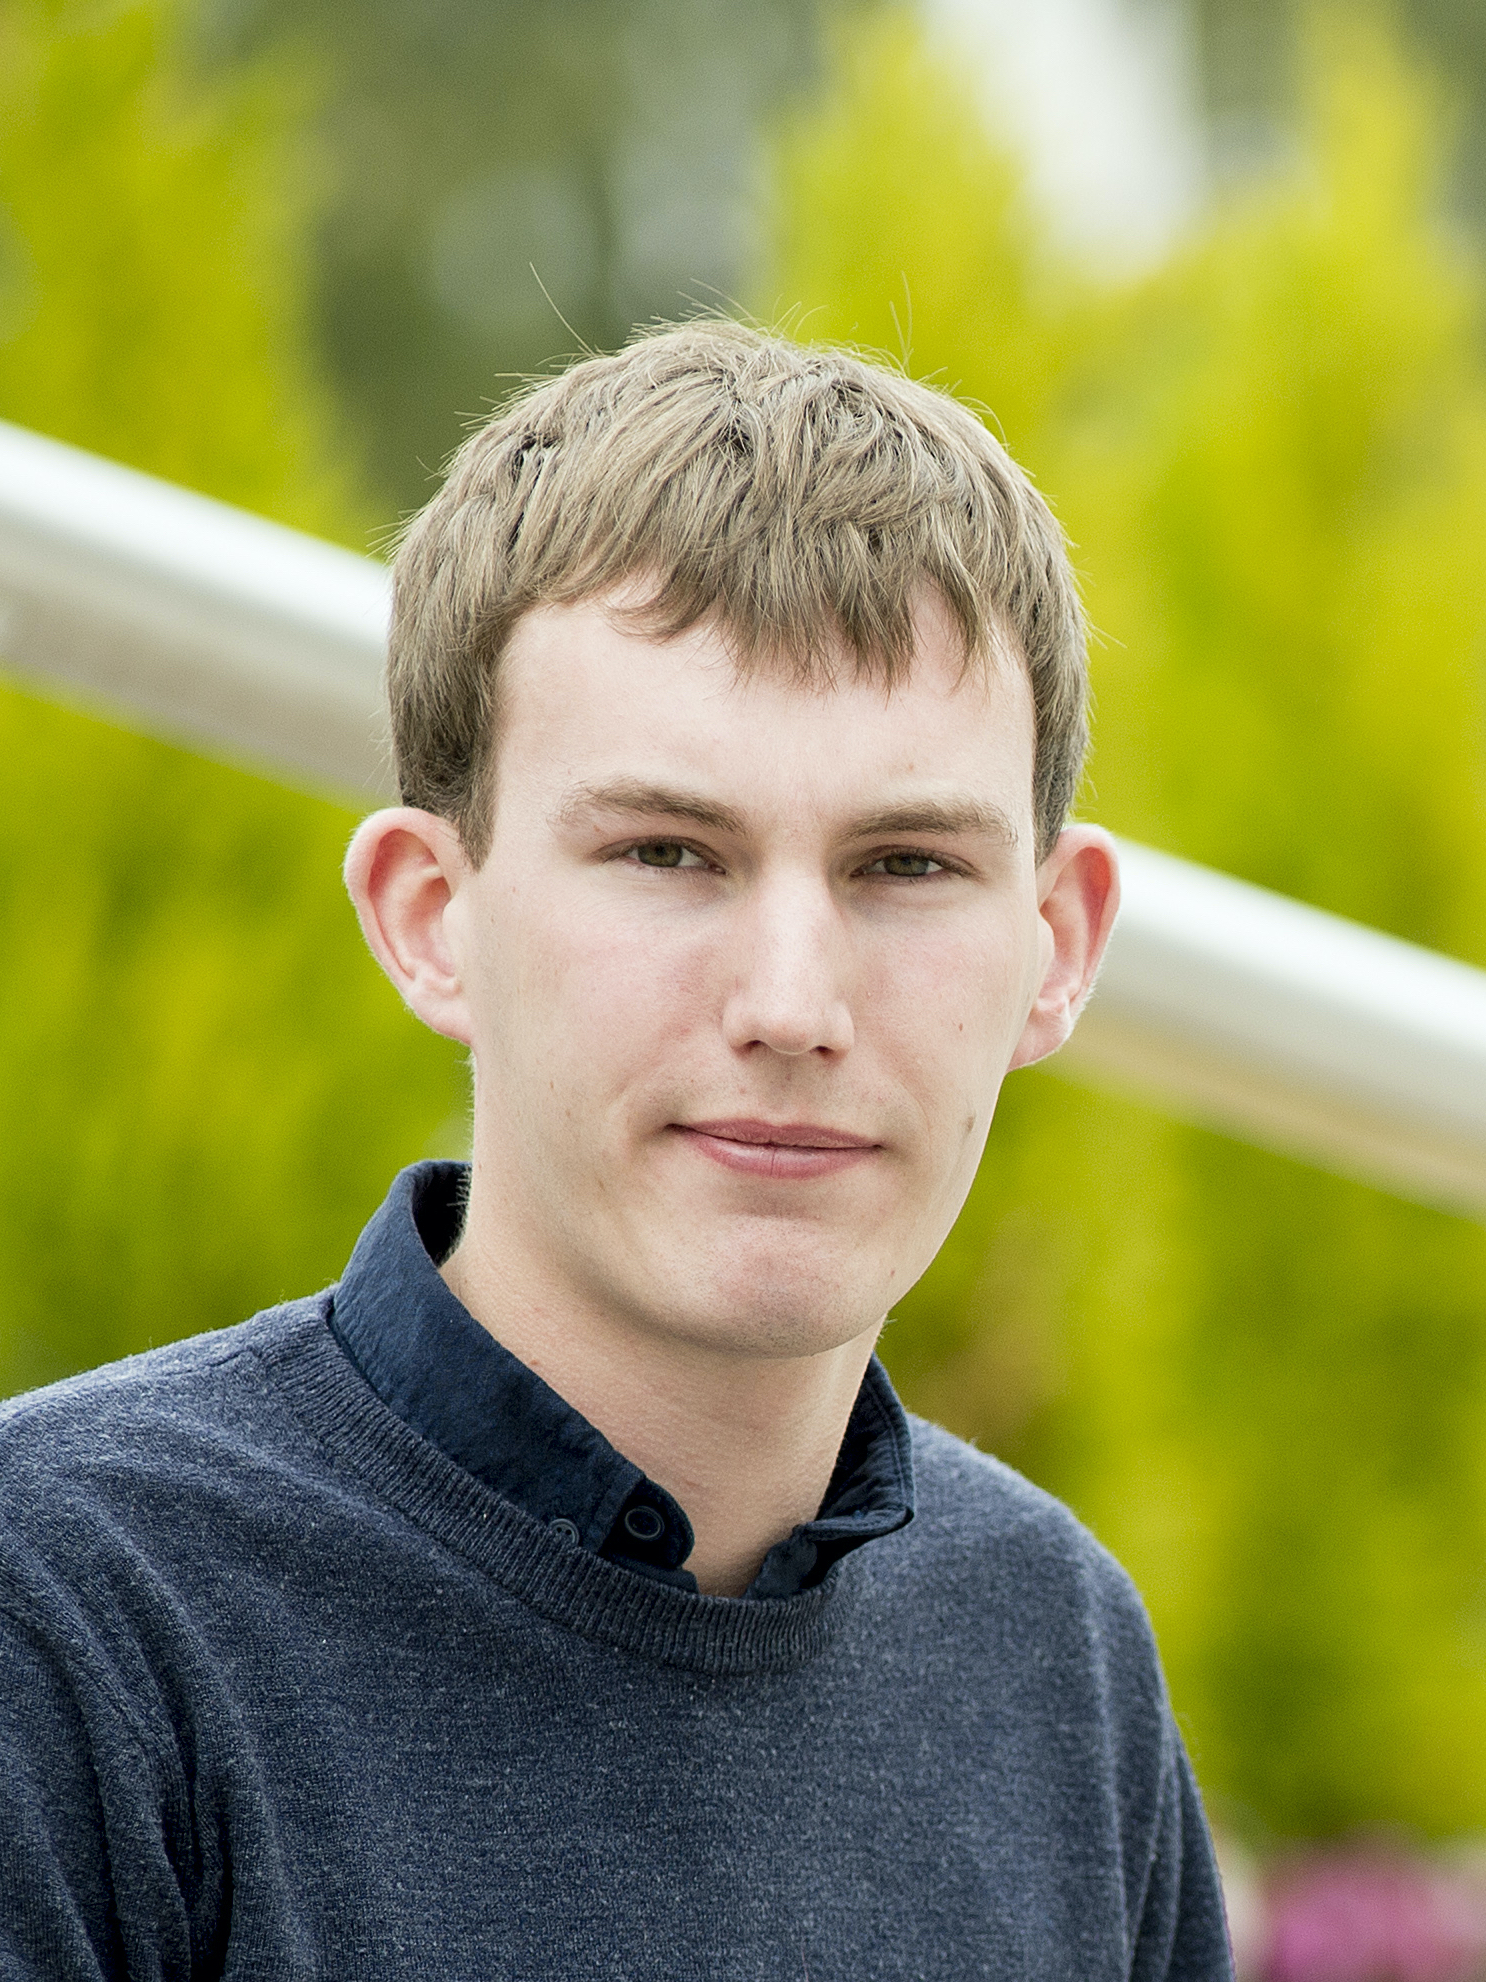
\includegraphics[width=30mm]{dp}\end{flushright}
}

\maketitlee

\href{https://lics.siglog.org/newsletters/}{Past Issues}
 - 
\href{https://lics.siglog.org/newsletters/inst.html}{How to submit an announcement}
\section{Table of Content}\begin{itemize}\item DEADLINES (\cref{deadlines}) 
 
\item CALLS 
 
\begin{itemize}\item CompLingInfoReasAI'21 (CALL FOR PAPERS) (\cref{CompLingInfoReasAI21})
\item CiE 2021 (CALL FOR INFORMAL PRESENTATIONS) (\cref{CiE2021})
\item CAV 2021 (CALL FOR STUDENT VOLUNTEERS) (\cref{CAV2021})
\item ETAPS 2022 (CALL FOR SATELLITE EVENTS) (\cref{ETAPS2022})
\item HIGHLIGHTS 2021 (CALL FOR CONTRIBUTED TALKS) (\cref{HIGHLIGHTS2021})
\item PODS 2022 (CALL FOR PAPERS) (\cref{PODS2022})
\item ESSLLI 2022 (CALL FOR COURSE AND WORKSHOP PROPOSALS) (\cref{ESSLLI2022})
\end{itemize} 
\item JOB ANNOUNCEMENTS 
 
\begin{itemize}\item Professor (W2) in “Knowledge Based Systems” at TU Dortmund University (\cref{ProfessorW2inKnowledgeBasedSystemsatTUDortmundUniversity})
\end{itemize} 
\end{itemize}\section{Deadlines}\label{deadlines}\rowcolors{1}{white}{gray!25}\begin{tabulary}{\linewidth}{LL}FSEN 2021:  & May 01, 2021 (Registration deadline) \\
VEST 2021:  & May 03, 2021 (Talk) \\
Professor (W2) TU Dortmund:  & May 5, 2021 (Application deadline) \\
ACM Transactions on Computational Logic:  & May 07, 2021 (Nominations for Editor-In-Chief) \\
VCLA Awards 2021:  & May 07, 2021 (Submission deadline, EXTENDED) \\
FCT 2021:  & May 09, 2021 (Abstract), May 16, 2021 (Paper) \\
FORMATS 2021:  & May 10, 2021 (Abstract+Paper EXTENDED) \\
RV 2021:  & May 13, 2021 (Abstract), May 20, 2021 (Paper) \\
CompLingInfoReasAI'21:  & May 14, 2021 (Paper) \\
CiE 2021:  & May 15, 2021 (Informal presentations) \\
CAV 2021:  & May 16, 2021 (Deadline for application for student volunteers) \\
FedCSIS’2021:  & May 24, 2021 (Paper) \\
ICGI 2020/21:  & May 25, 2021 (Paper) \\
ETAPS 2022:  & May 31, 2021 (Satellite event proposals deadline) \\
CALCO 2021:  & Jun 03, 2021 (Paper) \\
HIGHLIGHTS 2021:  & Jun 04, 2021 (Submission deadline (7pm GMT)) \\
PODS 2022:  & Jun 11, 2021 (First cycle abstract), Jun 18, 2021 (Full paper) \\
ESSLLI 2022:  & Jun 15, 2021 (Course Title), Jun 22, 2021 (Final) \\
EXPRESS/SOS 2021:  & Jun 21, 2021 (Paper) \\
ACKERMANN AWARD 2021:  & Jul 01, 2021 (Deadline for nomination) \\
CSL22:  & Jul 05, 2021 (Abstract), Jul 12, 2021 (Paper) \\
\end{tabulary}
\section{CompLingInfoReasAI'21: Computational Linguistics, Information, Reasoning, and AI 2021}\label{CompLingInfoReasAI21}  Salamanca, Spain, 6th-8th October, 2021, HYBRID  \\ 
  \href{https://www.dcai-conference.net/special-sessions/clirai}{https://www.dcai-conference.net/special-sessions/clirai}\\ 
CALL FOR PAPERS 

\begin{itemize}\item  SCOPE: 
 
  Computational and technological developments that incorporate natural language and reasoning methods are proliferating. Adequate coverage encounters difficult problems related to partiality, underspecification, agents, and context dependency, which are signature features of information in nature, natural languages, and reasoning. 
 
  The session covers theoretical work, applications, approaches, and techniques for computational models of information, language (artificial, human, or natural in other ways), reasoning. The goal is to promote computational systems and related models of thought, mental states, reasoning, and other cognitive processes. 
 
\item  TOPICS: 
 
  We invite contributions relevant to the following topics, without being limited to them, across approaches, methods, theories, implementations, and applications: 
 
\begin{itemize}\item  Theorem provers and assistants; Model checkers; Theory of computation; Theory of information; Computational methods of inferences in natural language; Computational theories and systems of reasoning in natural language; Transfer of reasoning in natural language to theorem provers, or vice versa; Transfer of reasoning between natural language, theorem provers, model checkers, and various computational assistants; Computational approaches of computational linguistics for domain specific areas; Theories for applications to language, information processing, reasoning; Type theories for applications to language, information processing, reasoning; Computational grammar; Computational syntax; Computational semantics of natural languages; Computational syntax-semantics interface; Interfaces between morphology, lexicon, syntax, semantics, speech, text, pragmatics; Parsing; Multilingual processing; Large-scale grammars of natural languages; Models of computation and algorithms for linguistics, natural language processing, argumentation; Computational models of partiality, underspecification, and context-dependency; Models of situations, contexts, and agents, for applications to computational linguistics; Information about space and time in language models and processing
\item  Data science in language processing; Machine learning of language and reasoning; Interdisciplinary methods; Integration of formal, computational, model theoretic, graphical, diagrammatic, statistical, and other related methods; Logic for information extraction or expression in written or spoken language; Logic for information integrations of diagrams, with written and / or spoken language
\item  Formal models of argumentations; Interactive computation, reasoning, argumentation; Computation with heterogeneous information; Reasoning with heterogeneous and/or inconsistent information; Dialog, interactions; Interdisciplinary approaches to language, computation, reasoning, memory; Argumentation in AI applications, e.g., to business, economy, justice, health, medical sciences
\item  Language processing based on biological fundamentals of information and languages; Computational neuroscience of language; etc.
\end{itemize} 
\item  PAPER SUBMISSION 
 
  \href{https://www.dcai-conference.net/special-sessions}{https://www.dcai-conference.net/special-sessions} 
 
  \href{https://www.dcai-conference.net/submission}{https://www.dcai-conference.net/submission} 
 
  The papers must be PDF format consist of original, relevant, and previously unpublished sound research results related to any of the topics of the Special Session CompLingInfoReasAI'21. 
 
  DCAI Special Session papers must be formatted according to the Springer AISC Template, with a maximum length of 10 pages in length, including figures and references.  
 
\item  PUBLICATION 
 
  All accepted, registered, and presented papers will be published by Advances in Intelligent Systems and Computing, AISC, series of Springer Verlag. At least one of the authors of an accepted paper will be required to register and attend the symposium to present the paper in order to include it in the conference proceedings. 
 
\item  IMPORTANT DATES 
 
\rowcolors{1}{white}{gray!25}\begin{tabulary}{\linewidth}{LL}Paper submission:  & May 14, 2021 \\
Notification of acceptance:  & Jun 07, 2021 \\
Camera-Ready papers:  & Jun 28, 2021 \\
Conference:  & Oct 6-8, 2021 \\
\end{tabulary}
 
\end{itemize}\section{CiE 2021: Connecting with computability}\label{CiE2021}  July 5–9, 2021, virtual\\ 
  \href{http://www.CiE2021.ugent.be}{http://www.CiE2021.ugent.be}\\ 
CALL FOR INFORMAL PRESENTATIONS 

\begin{itemize}\item  CiE 2021 is the seventeenth conference organized by the Association Computability in Europe. The /Computability in Europe/ conference (CiE) series has built up a  strong tradition for developing a scientific program which is interdisciplinary at its core bringing together all aspects of computability and foundations of computer science, as well as the interplay of these theoretical areas with practical issues in CS and other disciplines such as biology, mathematics, history, philosophy, and physics. For more information about the CiE conferences and the Association  CiE, please have a look at: \href{https://www.acie.eu/}{https://www.acie.eu/}. 
 
  CiE 2021 will be the second CiE conference that is organized as a virtual event and aims at a high-quality meeting that allows and invites active participation from all participants. It will be hosted virtually by Ghent University. 
 
\item   INFORMAL PRESENTATIONS: 
 
  Continuing the tradition of past CiE conferences, in addition to the formal presentations based on the LNCS proceedings volume, CiE 2021 will host a track of informal presentations, that are prepared very shortly before the conference and inform the participants about current research and work in progress.  The Programme Committee cordially invites all researchers (European and non-European) to submit their abstract for informal presentations. The abstract will be posted on the CiE 2021 website. 
 
  The deadline for the submission of abstracts for informal presentations is May 15, 2021. Informal presentations proposals should be at most one page PDF, submitted to: \href{https://easychair.org/conferences/?conf=cie2021}{https://easychair.org/conferences/?conf=cie2021} 
 
  Notification can be expected a few days after the submission deadline 
 
  Registration for CiE 2021 will be free (opening soon). 
 
\item  PLENARY SPEAKERS 
 
\begin{itemize}\item  Laura Crosilla (University of Oslo, Norway)
\item  Markus Lohrey (Universität Siegen. Germany)
\item  Russell Miller (tutorial speaker, CUNY, US)
\item  Joan Rand Moschovakis (Occidental College, emerita)
\item  Joël Ouaknine (Max Planck Institute for software systems, Germany)
\item  Christine Tasson (tutorial speaker, Université Paris Diderot, France)
\item  Keita Yokoyama (Japan Advanced Institute of Science and Technology, Japan)
\item  Henry Yuen (University of Toronto, Canada)
\end{itemize} 
\item  SPECIAL SESSIONS 
 
\begin{itemize}\item  Church's thesis in constructive mathematics (HaPoC session): Marianna Antonutti-Marfori (Ludwig-Maximilians-Universität München, Germany) and Alberto Naibo (Université Paris 1 Panthéon-Sorbonne)
\item  Classical Computability theory: Open problems and solutions: Noam Greenberg (Victoria University of Wellington, New Zealand) and Steffen Lempp (University of Wisconsin)
\item  Computational geometry: Maike Buchin (Ruhr-Universität Bochum, Germany) and Maarten Löffler (Utrecht University, Netherlands)
\item  Computational Pangenomics: Nadia Pisanti (University of Pisa, Italy) and Solon Pissis (University of Amsterdam, Netherlands)
\item  Proof theory and computation: David Fernández Duque (Ghent University, Belgium) and Juan Pablo Aguilera (Ghent University, Belgium)
\item  Quantum computation and information: Harry Buhrman (Universiteit van Amsterdam, Netherlands) and Frank Verstraete (Ghent University, Belgium)
\end{itemize} 
\item  WOMEN IN COMPUTABILITY 
 
  The Computability in Europe conference series has a long tradition in setting up a Women in Computability program. For CiE 2021 we plan a Women in Computability workshop combined with an online mentoring program. For more details on the Special Interest Group Women in Computability, see: \href{https://www.acie.eu/cie-conference-series/cie-cs-women-in-computability/}{https://www.acie.eu/cie-conference-series/cie-cs-women-in-computability/} 
 
\end{itemize}\section{CAV 2021: Computer-Aided Verification}\label{CAV2021}  \href{http://i-cav.org/2021/}{http://i-cav.org/2021/}\\ 
CALL FOR STUDENT VOLUNTEERS 

\begin{itemize}\item  The CAV 2021 Program for Student Volunteers provides an opportunity for students all around the world to attend and contribute to the 33rd International Conference on Computer-Aided Verification. 
 
  As a student volunteer, you will be working with peer students and the CAV organizing committee to help organize this year’s virtual conference. More details are described below. If you want to join, please do not hesitate to apply! 
 
\item  ELIGIBILITY 
 
  Applicants must be undergraduate, Master’s, Ph.D., full- or part-time students, studying computer science or related fields. Moreover, we expect applicants to: 
 
\begin{itemize}\item  Be able to attend at least 3 days of the conference during July 18 to 23, 2021.
\item  Be punctual, responsible, and self-motivated.
\item  Be available for pre-conference work (e.g. checking pre-recorded talks), preparation and/or training.
\end{itemize} 
  Student volunteers will mainly cover the following tasks during CAV 2021: 
 
\begin{itemize}\item  Help with conference scheduling.
\item  Check and edit pre-recorded video talks.
\item  Help organize virtual talks and Q\&A sessions.
\item  Help manage the conference’s chat channels and other virtual social activities.
\item  Assist with publicity on social media.
\end{itemize} 
\item  BENEFITS  
 
  As a student volunteer you will get: 
 
\begin{itemize}\item  Free full registration of CAV 2021 and its associated workshops.
\item  A virtual student volunteers dinner (covered by Uber Eats vouchers)
\item  Chance to meet and network with both researchers and peer students in the field of computer-aided formal verification.
\end{itemize} 
\item  APPLICATION 
 
\rowcolors{1}{white}{gray!25}\begin{tabulary}{\linewidth}{LL}Deadline for application for student volunteers:  & May 16, 2021 \\
Notification:  & May 23, 2021 \\
\end{tabulary}
 
  \href{http://i-cav.org/2021/sv-signup}{http://i-cav.org/2021/sv-signup}.  
 
\end{itemize}\section{ETAPS 2022: 25th European Joint Conferences on Theory and Practice of Software }\label{ETAPS2022}  Munich, Germany, April 2-7, 2022\\ 
CALL FOR SATELLITE EVENTS 

\begin{itemize}\item  ABOUT ETAPS 
 
  The European Joint Conferences on Theory and Practice of Software  (ETAPS) is the primary European forum for academic and industrial researchers working on topics relating to Software Science. It is an annual event held in Europe each spring since 1998. Its twenty-fifth edition, ETAPS 2022, will take place April 2-7, 2022, in Munich, Germany.  
 
  ETAPS 2022 main conferences, scheduled for April 4-7, are:  
 
\begin{itemize}\item  ESOP: European Symposium on Programming 
\item  FASE: Fundamental Approaches to Software Engineering 
\item  FOSSACS: Foundations of Software Science and Computation Structures 
\item  TACAS: Tools and Algorithms for the Construction and Analysis of Systems 
\end{itemize} 
\item  SATELLITE EVENTS 
 
  The ETAPS 2022 organizing committee invites proposals for satellite events (workshops) to complement the main conferences. They should fall within the scope of ETAPS. The topics encompass all aspects of the system development process, including specification, design, implementation, analysis, improvement, the languages, methodologies, and tools that support these activities, covering a spectrum from practically motivated theory to soundly-based practice. 
 
  Satellite events provide an opportunity to discuss and report on emerging research approaches and practical experience relevant to the theory and practice of software.  
 
  ETAPS 2022 satellite events will take place immediately before the main conferences, on April 2-3. 
 
\item  ARRANGEMENTS FOR SATELLITE EVENTS 
 
  The organizers of an ETAPS 2022 satellite are expected to: 
 
\begin{itemize}\item  create and maintain a website for the event
\item  form a PC, produce a call for papers for the event (if appropriate), 
\item  advertise the event through specialist mailing lists etc. to complement the publicity of ETAPS, 
\item  review the submissions received and make acceptance decisions, 
\item  prepare an informal (pre)proceedings for the event (if appropriate), 
\item  design the event's program complying with any scheduling constraints defined by the ETAPS 2022 organizing committee, 
\item  prepare and organize the publication of formal (post)proceedings (if desired). 
\end{itemize} 
  As a rule, ETAPS will not contribute toward the travel or accommodation costs of invited speakers or satellite events organizers.  
 
\item  SUBMISSION OF SATELLITE EVENT PROPOSALS 
 
  Researchers and practitioners wishing to organize satellite events are invited to submit proposals via the following online form (courtesy of Rob van Glabbeek): \href{http://eptcs.web.cse.unsw.edu.au/ETAPS/}{http://eptcs.web.cse.unsw.edu.au/ETAPS/}  
 
  Please see the full call: \href{https://etaps.org/2022/call-workshop-proposals}{https://etaps.org/2022/call-workshop-proposals} for the responsibilities of the  The ETAPS 2022 organizing committee and the required information. 
 
  The ETAPS 2022 organizing committee will evaluate the proposals based on their assessed benefit for prospective participants of ETAPS 2022.  
 
\item  FURTHER INFORMATION AND ENQUIRIES 
 
  Please contact the Etaps'22 workshop chair Dirk Beyer dirk.beyer@lmu.de or the general chair Jan Kretinsky jan.kretinsky@tum.de 
 
\item  IMPORTANT DATES 
 
\rowcolors{1}{white}{gray!25}\begin{tabulary}{\linewidth}{LL}Satellite event proposals deadline:  & May 31, 2021 \\
Notification of acceptance:  & Jun 10, 2021 \\
\end{tabulary}
 
\end{itemize}\section{HIGHLIGHTS 2021: 9th annual conference on Highlights of LOGIC, GAMES, and AUTOMATA}\label{HIGHLIGHTS2021}  15-17 September 2021, Aachen (but most probably online)\\ 
  \href{http://highlights-conference.org}{http://highlights-conference.org}\\ 
CALL FOR CONTRIBUTED TALKS 

\begin{itemize}\item  HIGHLIGHTS 2021 is the 9th conference on Highlights of Logic, Games, and Automata that aims to integrate the diverse research community working in the areas of Logic, Finite Model Theory, Automata Theory, Games and Verification. Individual papers are dispersed across many conferences, which makes them challenging to follow. Participating in the annual Highlights conference offers a wide picture of the latest research in the field and a chance to meet and interact with most of the members of the research community. The speakers are encouraged to present their best recent work at Highlights, whether already published elsewhere or not. We invite submissions for contributed talks (around 10 minutes). 
 
  There will be a tutorial day (14 September) and three days for the conference (15-17 September).  
 
  This year's edition will be most probably held online, with no registration fees. 
 
\item  Submission instructions and more detailed information about the conference to be found at \href{http://highlights-conference.org}{http://highlights-conference.org} 
 
\item  TUTORIALS (September 14) 
 
\begin{itemize}\item  Christoph Haase
\item  Michał Pilipczuk
\end{itemize} 
\item  KEYNOTES 
 
\begin{itemize}\item  Rajeev Alur
\item  Balder ten Cate
\item  Karoliina Lehtinen
\item  Nutan Limaye
\item  Joel Ouaknine
\end{itemize} 
\item  IMPORTANT DATES: 
 
\rowcolors{1}{white}{gray!25}\begin{tabulary}{\linewidth}{LL}Submission deadline (7pm GMT):  & Jun 04, 2021 \\
Notification (7pm GMT):  & Jun 18, 2021 \\
\end{tabulary}
 
\end{itemize}\section{PODS 2022: 41st ACM SYMPOSIUM ON PRINCIPLES OF DATABASE SYSTEMS}\label{PODS2022}  \href{https://databasetheory.org/node/125}{https://databasetheory.org/node/125}\\ 
CALL FOR PAPERS 

\begin{itemize}\item  SCOPE: PODS seeks high-quality scientific articles that present principled contributions to modeling, application, system building, and both theoretical and experimental validation in the context of data management. Such articles might be based, among others, on establishing theoretical results, developing new concepts and frameworks that deserve further exploration, providing experimental work that sheds light on the scientific foundations of the discipline, or a rigorous analysis of both widely used and recently developed industry artifacts.  
 
\item  TOPICS OF INTEREST: Topics that fit the interests of the symposium include, but are not limited to, database design (data models, query languages, schemas, constraints), database access (data structures, access methods, concurrency, transactions), data quality (data cleaning, data discovery, data exploration), database processing (query evaluation, query optimization, schema management, distributed data processing, approximate data processing), data analysis (data mining, machine learning, information extraction, data streams), uncertainty (incompleteness, inconsistency, ontological query answering, semi-structured data), interoperability (mappings and views, data integration, data exchange, ontology-based data access, responsible data management (access control, privacy, security, verification, ethical aspects of data management), dynamics of  data (workflows, data-centric process management, web services, data provenance, incremental query evaluation) 
 
\item  IMPORTANT DATES:  
 
  Dates for the first submission cycle are as follows.  
 
\rowcolors{1}{white}{gray!25}\begin{tabulary}{\linewidth}{LL}First cycle abstract submission:  & Jun 11, 2021 \\
Full paper submission:  & Jun 18, 2021 \\
Reviews sent to authors:  & Jul 31, 2021 \\
Rebuttal phase:  & Aug 1-5, 2021 \\
Notification:  & Aug 13, 2021 \\
\end{tabulary}
 
\end{itemize}\section{ESSLLI 2022: 33rd European Summer School in Logic, Language and Information }\label{ESSLLI2022}  8-19 August, 2022, Galway, Ireland\\ 
  \href{https://2022.esslli.eu/}{https://2022.esslli.eu/}\\ 
CALL FOR COURSE AND WORKSHOP PROPOSALS 

\begin{itemize}\item  Under the auspices of the Association for Logic, Language, and Information (FoLLI), the European Summer School in Logic, Language, and Information (ESSLLI) runs every year. Except for 2021, where the school will be virtual, it runs in a different European country each year. It takes place over two weeks in the summer, hosts approximately 50 different courses at both introductory and advanced levels, and attracts around 400 participants from all over the world. 
 
  Since 1989, ESSLLI has been providing outstanding interdisciplinary educational opportunities in the fields of Computer Science, Cognitive Science, Linguistics, Logic, Philosophy, and beyond. It comes from a community which recognizes that advances in our common areas require the contributions of multiple interrelated disciplines. 
 
  The main focus of ESSLLI is the interface between linguistics, logic and computation, with special emphasis in human linguistic and cognitive ability. Courses, both introductory and advanced, cover a wide variety of topics within the combined areas of interest: Logic and Computation, Computation and Language, and Language and Logic. Workshops are also organized, providing opportunities for in-depth discussion of issues at the forefront of research, as well as a series of invited evening lectures. 
 
\item  TOPICS AND FORMAT  
 
  Proposals for courses and workshops at ESSLLI 2022 are invited in all areas of Logic, Linguistics and Computer Sciences. Cross-disciplinary and innovative topics are particularly encouraged. 
 
  Each course and workshop will consist of five 90 minute sessions, offered daily (Monday-Friday) in a single week. Proposals for two-week courses should be structured and submitted as two independent one-week courses, e.g. as an introductory course followed by an advanced one. In such cases, the ESSLLI program committee reserves the right to accept just one of the two proposals. 
 
  All instructional and organizational work at ESSLLI is performed completely on a voluntary basis, so as to keep participation fees to a minimum. However, organizers and instructors have their registration fees waived, and are reimbursed for travel and accommodation expenses up to a level to be determined and communicated with the proposal notification. ESSLLI can only guarantee reimbursement for at most one course/workshop organizer, and can not guarantee full reimbursement of travel costs for lecturers or organizers from outside of Europe. The ESSLLI organizers would appreciate any help in controlling the School's expenses by seeking partial or complete coverage of travel and accommodation expenses from other sources. 
 
\item  CATEGORIES: each proposal should fall under one of the following categories. 
 
\begin{itemize}\item  FOUNDATIONAL COURSES: Such courses are designed to present the basics of a research area, to people with no prior knowledge in that area. They should be of elementary level, without prerequisites in the course's topic, though possibly assuming a level of general scientific maturity in the relevant discipline. They should enable researchers from related disciplines to develop a level of comfort with the fundamental concepts and techniques of the course's topic, thereby contributing to the interdisciplinary nature of our research community.
\item  INTRODUCTORY COURSES: Introductory courses are central to ESSLLI's mission. They are intended to introduce a research field to students, young researchers, and other non-specialists, and to foster a sound understanding of its basic methods and techniques. Such courses should enable researchers from related disciplines to develop some comfort and competence in the topic considered. Introductory courses in a cross-disciplinary area may presuppose general knowledge of the related disciplines.
\item  ADVANCED COURSES: Advanced courses are targeted primarily to graduate students who wish to acquire a level of comfort and understanding in the current research of a field.
\item  WORKSHOPS: Workshops focus on specialized topics, usually of current interest. Workshop organizers are responsible for soliciting papers and selecting the workshop program. They are also responsible for publishing proceedings if they decide to have proceedings. 
\end{itemize} 
\item  PROPOSAL GUIDELINES 
 
  Course and workshop proposals should closely follow these guidelines to  ensure full consideration. 
 
   Course and Workshop proposals can be submitted by no more than two lecturers/organizers and they are presented by no more than these two lecturers/organizers. All instructors and organizers must possess a PhD or equivalent degree by the submission deadline. 
 
  Course proposals should mention explicitly the intended course category. Proposals for introductory courses should indicate the intended level, for example as it relates to standard textbooks and monographs in the area. Proposals for advanced courses should specify the prerequisites in detail.  
 
  Proposals of Courses given at ESSLLI the previous year will have a lower priority of being accepted in the current year. Proposals must be submitted in PDF format via: \href{https://easychair.org/conferences/?conf=esslli2022}{https://easychair.org/conferences/?conf=esslli2022} and include all of the following: 
 
\begin{itemize}\item  Personal information for each proposer: Name, affiliation, contact address, email, homepage (optional)
\item  General proposal information: Title, category
\item  Contents information: Abstract of up to 150 words, Motivation and description (up to two pages), Tentative outline, Expected level and prerequisites, Appropriate references (e.g. textbooks, monographs, proceedings, surveys)
\item  Information on the proposer and course: Will your course appeal to students outside of the main discipline of the course? Include information on your experience in the intensive one-week interdisciplinary setting Include evidence that the course proposer is an excellent lecturer.
\item  Information from workshop organizers: Include information on relevant preceding meetings and events, if  applicable Include information about potential external funding for participants.
\end{itemize} 
\item  SUBMISSION INFORMATION  
 
\begin{itemize}\item  By June 15: You are asked to submit in EasyChair at least the name(s) of the instructor(s),  the ESSLLI area+course level and a short abstract.
\item  By June 22: Your submission must be completed by uploading a PDF with the actual proposal  as detailed above.
\end{itemize} 
\item  CHILDCARE:  If there is enough interest, ESSLLI will provide information on private child care services available during the summer school. 
 
\item  EACSL SPONSORSHIP  
 
  The EACSL will support one Logic and Computation course or workshop addressing topics of interest to Computer Science Logic (CSL) conferences. The selected course or workshop will be designated an EACSL course/workshop in the programme. If you wish to be considered for this, please indicate so in your proposal. 
 
\item  IMPORTANT DATES: 
 
\rowcolors{1}{white}{gray!25}\begin{tabulary}{\linewidth}{LL}Course Title submission:  & Jun 15, 2021 \\
Final submission:  & Jun 22, 2021 \\
Notification:  & Sep 14, 2021 \\
\end{tabulary}
 
\end{itemize}\section{Professor (W2) in “Knowledge Based Systems” at TU Dortmund University}\label{ProfessorW2inKnowledgeBasedSystemsatTUDortmundUniversity}JOB ANNOUNCEMENT 

\begin{itemize}\item  The Department of Computer Science at TU Dortmund University is seeking to fill the position of a Professor (W2) in “Knowledge Based Systems” commencing as soon as possible. The successful candidate will specialize in research and teaching in the field of “Knowledge Based Systems”. TU Dortmund University is seeking an outstanding individual and well established researcher in the field of “Knowledge Based Systems” with a focus on Knowledge Representation and Reasoning and with relevant international publications in recognized venues with peer-review. Applicants should complement the research activities of the Department of Computer Science and contribute to interdisciplinary collaborative research projects within and outside TU Dortmund University. 
 
  An appropriate contribution to the department’s core curriculum, especially in the area of logic is required, in the medium term also in German. The successful candidate will possess social and leadership skills and be willing to be involved in academic self-governance. Preconditions for employment are specified in § 36 and § 37 HG NRW (law governing universities in North-Rhine Westphalia). 
 
\item  With 6,500 employees in research, teaching and administration and its unique profile, TU Dortmund University shapes prospects for the future: the interaction between engineering and natural sciences as well as social and cultural studies drives both technological innovations and progress in knowledge and methodology. It is not only the roughly 33,400 students who benefit from this. The Department of Computer Science at TU Dortmund University is one of the largest in Germany, with particular strengths in research. Among similar institutions it is distinguished by a combination of fundamental research on formal methods with the development of practical applications.Research focuses on Algorithmics, Data Science, Cyber-Physical Systems, and Software and Service Engineering. 
 
\item  TU Dortmund University strives to increase the number of women in academic research and teaching and therefore explicitly encourages women to apply. TU Dortmund University is an equal opportunity employer and gives preference to candidates with disabilities if equally qualified. TU Dortmund University supports the compatibility of work and family life and promotes gender equality in science. 
 
\item  Please send your application, including the usual documents (CV, list of publications, certificates, etc.) preferably by e-mail (in one pdf-file) to the following address by 05.05.2021: 
 
  Dean of the Department of Computer Science, Professor Dr.-Ing. Gernot A. Fink 
 
  TU Dortmund University 
 
  44221 Dortmund – Germany 
 
  tel: 0049-231/755-6151 
 
  fax: 0049-231/755-6116 
 
  e-mail: bewerbung@cs.tu-dortmund.de 
 
  \href{http://www.cs.tu-dortmund.de/}{http://www.cs.tu-dortmund.de/} 
 
  Questions can be also addressed to thomas.schwentick@tu-dortmund.de. 
 
\item  FULL ADVERT 
 
  \href{https://service.tu-dortmund.de/documents/18/2120803/Professor+W2+in+Knowledge+Based+Systems.pdf/b887f51b-8ba1-16bf-1aa7-3d7907e84d54}{https://service.tu-dortmund.de/documents/18/2120803/Professor+W2+in+Knowledge+Based+Systems.pdf/b887f51b-8ba1-16bf-1aa7-3d7907e84d54} 
 
\end{itemize}


To the \href{http://siglog.org/}{SIGLOG} or \href{https://lics.siglog.org}{LICS} website\end{document}